\section{Methods}
There are many existing language learning software, which, fall into two categories, learning by  
lessons and learning vocabularies. In the first category, 
%learning in lessons, they manually design some lessons to help their 
lessons are purposefully designed to help users easily learn a foreign language.
Duolingo\footnote{\url{https://www.duolingo.com/}} is a popular websites in this category. 
For the second categoryusers are guided to recite lists of words, or provided with a translation for their input word in the foreign language.Google Translate \footnote{\url{https://translate.google.com/}} stands out in this category. The service is available as desktop / mobile / web software including a chrome extension. We mainly compare our system  with the aforementioned two softwares.
Table~\ref{table:difference_summary} summarises important differences between 
our system and all these existing tools. Each difference serves as a motivation 
for developing our extension.
\\
``Duolingo is a free language-learning and crowdsourced text translation 
platform''\footnote{\url{http://en.wikipedia.org/wiki/Duolingo}}.
Most people start to use Duolingo when they know a little or nothing about 
the new language. They starting from some basic lessons and improve step by step.
However, our target audience 
is a mix novice and intermediate level learners of the foreign language. 
We can not only help beginners learn 
a new language but also help them continue their learning by allowing them to practice 
their foreign language. There are also a lot articles with their translations in 
Duolingo, but all the articles and their translations are manually added by 
Duolingo or users from Duolingo. Therefore, parallel articles in Duolingo are old and 
limited. However, our chrome extension is always working even for those up to the 
minute news and our user can just practice their foreign language in their daily 
readings.

\textbf{Google Translate:} ``Highlight or right-click on a section of text and click
on Translate icon next to it to translate it to your 
language''\footnote{\url{http://en.wikipedia.org/wiki/Google_Chrome_Extensions}}. 
% Tao: please cite
Google Translate is a chrome extension that displays only the translation when user 
select a section, which can be a word, a phrase, a sentence or even a whole page. 
Our chrome extension will translate a single word only, and display the translation,
following with the pronunciations and example sentences to help user understand and 
remember this word. Compared with our extension, Google Translate is more like an extension 
to help user understand the content of the page. Furthermore, our extension will display 
the most appropriate translation as it will refer to the context of the word.
\begin{table}[ht]
  \caption{Summary of the differences}
  \label{table:difference_summary}
  \begin{center}
  \begin{tabular}{| p{2.4cm} | p{1.2cm} | p{1.2cm} |  p{1.2cm} |}
    \hline
    & Duolingo & Google Translate & Chrome Extension \\
    \hline
    Lessons & Yes & No & No \\
    \hline
    User's foreign language level & Low & Low-High & Low-High \\
    \hline
    Time consuming & Yes & No & No\\
    \hline
    Resource & Limited & Infinite & Infinite \\
    \hline
    Customizable & Yes & No & Yes \\
    \hline
    Link to External Dictionary & No & No & Yes \\
    \hline
  \end{tabular}
  \end{center}
\end{table}
\subsection{Software Design}
Based on the user study, we divided the extension into three components: translating, learning and testing. After user opened a news website, 
some words in the main content will be replaced by their translation from user's preferred foreign language, and this is what our translating 
component is doing. If user want to know more about the replaced word, he can simply move his mouse over the translation and a window will pop 
over to help user learn this word, and this is learning component. If user have encountered some word for a few times, we will generate some 
quiz for him and this is testing component.
\subsubsection{Translating}
\begin{figure}[ht]
  \centering
  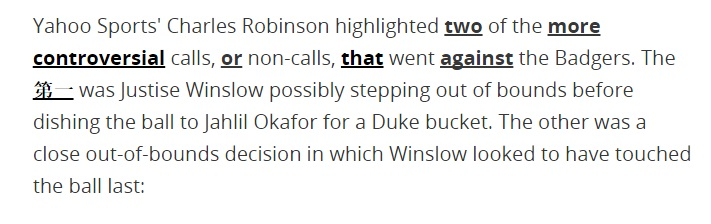
\includegraphics[width=0.45\textwidth]{software_design_2.jpg}
  \caption{Screen shot of Translating Component}
  \label{fig:software_design_2}
\end{figure}
After the original web page, our chrome extension will fetch the content of the news and pass them to the server paragraph by paragraph. After receiving the content, server will compare every word in the paragraph with the words in our vocabulary. If there are some matches, which simply means there are some words that need to be replaced. As every English word might have a few Chinese meanings, our server must select the most appropriate translation among all the meanings. The way that we are trying to solve this problem so far is to compare all the Chinese meanings with the translation of the whole sentence from Bing Translate. If any of the Chinese meanings is the substring of the translation of the sentence, our server will choose that meaning (This is not a proper and accurate way to solve this problem, but it is much better than randomly choose one Chinese meanings. Also, this would be my main research problem that I need to solve next semester). Then, server will pass a JSON string that contains all the words that need to be replaced, their Chinese meanings as well as their pronunciations back to front end. Then, front end will replace the content of the news paragraph by paragraph, in which some words have been replaced. Figure \ref{fig:software_design_2} is the screen shot of this component.
\\
\subsubsection{Learning}
\begin{figure}[ht]
  \centering
    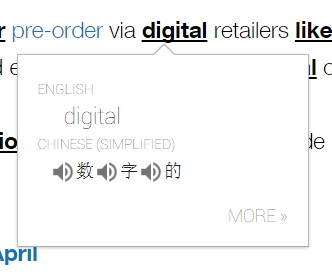
\includegraphics[width=0.3\textwidth]{software_design_4.jpg}
  \caption{Screen shot of popover with highlighted English word}
  \label{fig:software_design_4}
\end{figure}

\begin{figure}[ht]
    \centering
    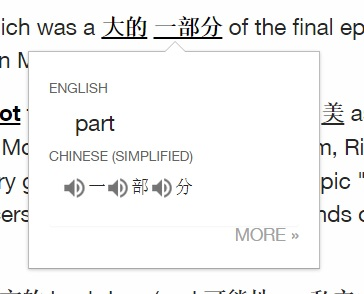
\includegraphics[width=0.3\textwidth]{software_design_5.jpg}
    \caption{Screen shot of popover with highlighted Chinese word}
    \label{fig:software_design_5}
\end{figure}
\\
By moving mouse on the Chinese word for one second, a window with its English meaning and pronunciation will pop over. Figure \ref{fig:software_design_4} is the screen shot of the pop over without its example sentence. If user want to know how to use this word, he can just click the button next to the pronunciation to get the example sentences of this word. After user click the button to get example sentence, our extension will send a request to server and wait for server' response. There is another way of doing this, which is simply get the example sentences together with the words in the Translating component. However, the example sentences contains much more characters comparing with the pronunciation. We want to maximize the loading speed and minimize the data transferred between front end and server, so we decided to split the pop over content into two request. Figure \ref{fig:software_design_5} is the screen shot of the pop over with its example sentences.
\\
\subsubsection{Testing}
\begin{figure}[ht]
\centering
  \centering
  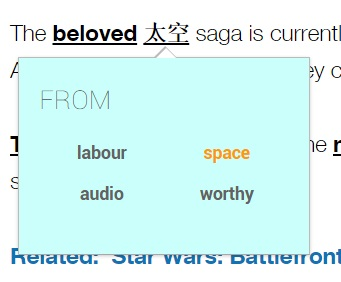
\includegraphics[width=0.3\textwidth]{software_design_7.jpg}
  \caption{Screenshot of English test popover}
  \label{fig:software_design_7}
\end{figure}

\begin{figure}[ht]
    \centering
  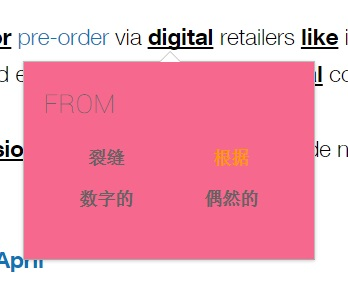
\includegraphics[width=0.3\textwidth]{software_design_8.jpg}
  \caption{Screen shot of Chinese test popover}
  \label{fig:software_design_8}
\end{figure}
When user has encountered the same word for a few times, our system will generate a quiz about this word for him.  If user move mouse over this replaced word, a window with a quiz will pop over. After user select one option, this window will tell user the correct answer and sent whether the answer is correct to server. Figure \ref{fig:software_design_7} is the screen shot of our testing popover in English. Figure \ref{fig:software_design_8} is the screen shot of our testing popover in Chinese.
